\begin{figure}
  \begin{center}
    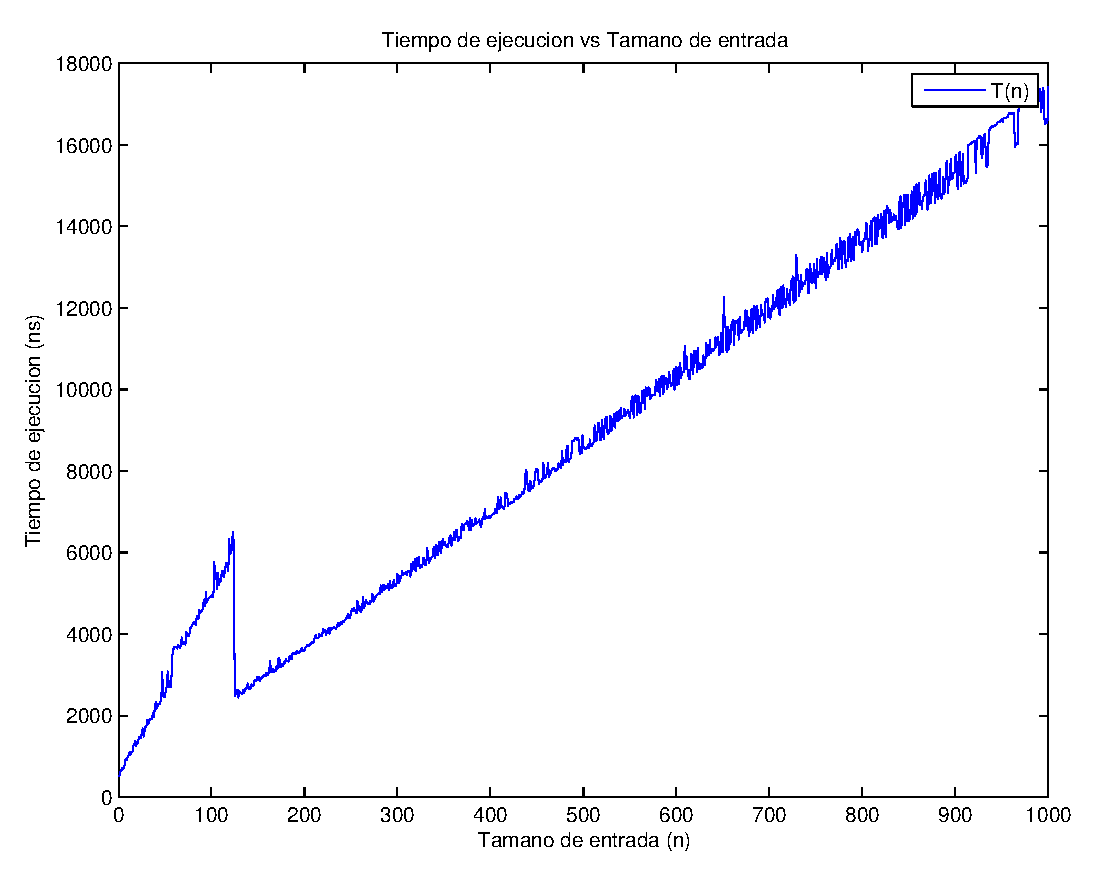
\includegraphics[scale=0.5]{problema1/graficos/problema1_aleatoria_1000.eps}
  \end{center}
  \caption{Caption}
  \label{fig:}
\end{figure}

Para concluir, nos parece importante destacar que la complejidad temporal de la solución es dominada por el algoritmo de ordenamiento. Esto implica que nuestra solución por más que la intentemos mejorar, no va a ser posible. Sin embargo, cabe destacar que en el caso en que los datos están ordenados al momento de leer, podemos mejorar la complejidad temporal de $O(n * log n)$ a $O(n)$.